\section{Introduction}
\label{sec:introduction}

Denote the set of nonnegative integers by $\NN$, and the set of positive integers by $\PP$. Given $N\in \NN$ and a set $\A$, together with a set-valued function $D:\A\to 2^{[N-1]}$ which is sometimes called a \emph{statistic}, we define its quasisymmetric generating function
\[
    \Q_{D} (\A) = \sum_{a \in \A} F_{N, D(a)},
\]
where $F_{N, S}$ is the \emph{fundamental quasisymmetric function} introduced by Gessel~\cite{knuth_classes_schur_positive}, indexed by a subset $S \subseteq [N-1]$ (see Section~\ref{subsec:definitions symmetric functions} for more background). We write $\Q(\A)$ instead of $\Q_{D}(\A)$ when $D$ is clear from the context.
The following long-standing problem was first addressed in~\cite{gessel1993counting}.
\begin{problem}[Gessel and Reutenauer]
    Find sets $\A$ and statistics $D$ for which $\Q_{D}(\A)$ is symmetric.
\end{problem}

When $\Q_{D}(\A)$ is symmetric, we say that $\A$ is symmetric with respect to the statistic $D$ (we omit $D$ when it is clear from the context). If $\A$ is symmetric, then there is a unique expansion
\[
    \Q_{D} (\A) = \sum_{\lambda \vdash N} c_\lambda s_\lambda,
\]
where $c_\lambda \in \QQ$ and $s_\lambda$ are Schur functions (discussed in Section~\ref{subsec:definitions symmetric functions}). The coefficients $c_\lambda$ are called the \emph{Schur coefficients} of $\A$.
If $c_\lambda \in \NN$ for all $\lambda \vdash N$, we say that $\A$ is Schur-positive with respect to $D$.

Gessel and Reutenauer also addressed the following problem:
\begin{problem}
    Find Schur-positive sets $\A$.
\end{problem}






The study of symmetric functions is partially motivated by the correspondence between symmetric functions of degree $N$ and class functions on the symmetric group $S_N$, which is established through the Frobenius characteristic map described in~\cite[Chapter 4.7]{sagan_book}. A symmetric function is Schur-positive if its corresponding class function is a proper character (see~\cite{adin_roichman_fine_set} for a detailed explanation). This perspective provides a rich algebraic framework for studying symmetric and Schur-positive sets.

During the last few decades, many Schur-positive subsets of the symmetric group $S_N$ were constructed with respect to the standard descent function of $S_N$, where a permutation $\pi \in S_N$ has $i \in \Des(\pi)$ if and only if $\pi(i) > \pi(i+1)$. A fundamental construction is due to Gessel~\cite{knuth_classes_schur_positive}, who proved that every set of permutations which is closed under the Knuth equivalence relations is Schur-positive. Furthermore, he showed that every Knuth class $\A \subset S_N$ (\ie equivalence class of the Knuth relations) satisfies $\Q_{\Des}(\A) = s_\lambda$ for some $\lambda \vdash N$. This result has many direct consequences. For example, for every $J \subseteq [N-1]$, the set $D_{N,J}^{-1} = \{ \pi^{-1} \mid \Des(\pi)=J\} \subseteq S_N$ is Schur-positive because it is closed under the Knuth relations.

Other examples of Schur-positive sets of permutations include all conjugacy classes, as proven by Gessel and Reutenauer~\cite{gessel1993counting}, and the set of permutations $\pi \in S_N$ with a fixed number of inversions (\ie $i<j$ such that $\pi(i) > \pi(j)$), a result demonstrated by Adin and Roichman \cite[Prop.\ 9.5]{adin_roichman_fine_set}.

Some Schur-positive sets that do not consist of permutations were found as well. For instance, Gessel~\cite{knuth_classes_schur_positive} proved that for every partition $\lambda \vdash N$, the set $\Syt(\lambda)$ of standard Young tableaux of shape $\lambda$ is Schur-positive (see Section~\ref{subsec:schur positive sets} for details).

In this work, we focus on the set of matchings of a given set of vertices.
\begin{definition}
\label{def:matching}
    A matching $m$ on a finite set of vertices $S \subseteq \PP$ is an unordered partition of $S$ into blocks, each block of size $1$ or $2$. If a block of a matching $m$ contains only the vertex $i$, we say that $i$ is an \emph{unmatched vertex} of $m$ and denote $(i) \in m$. If a block contains both $i$ and $j$ for $i<j$, we say that $(i,j)$ is a \emph{chord} of $m$ and denote $(i,j) \in m$. That is, the notation $(i,j)\in m$ implies that $i<j$. When $(i,j) \in m$, we also say that $i$ opens this chord and $j$ closes it. If a matching $m$ has no unmatched vertex, then we say that $m$ is a perfect matching.
\end{definition}

We will focus on matchings on the set $[N] := \{1,\dots, N\}$ for some $N \in \NN$. Denote by $\M_N$ the set of matchings on $[N]$, and by $\M_{N,f}$ the set of matchings on $[N]$ with $f$ unmatched vertices.

For example, 
\[
    \M_{4,0} = \big\{\{(1,2),\; (3,4)\},\ \{(1,3),\; (2,4)\},\ \{(1,4),\; (2,3)\}\big\}
\]
and
\[ 
    \M_{3,1} = \big\{\{(1,2),\; (3)\},\ \{(1,3),\; (2)\},\ \{(1),\; (2,3)\}\big\}.
\]

\begin{definition}
\label{def:intersect}
    Let $m$ be a matching on $S$. If $(i_1, i_3),\: (i_2,i_4) \in m$ for $i_1 < i_2 < i_3 < i_4$ then we say that the chords $(i_1, i_3)$ and $(i_2, i_4)$ \emph{intersect}.
\end{definition}

\begin{definition}
\label{def:short}
    Let $m \in \M_N$ be a matching on $[N]$. If $(i,i+1) \in m$, then it is called a \emph{short chord}. We denote $\Short(m) := \{i \in [N-1] \mid (i,i+1) \in m\}$.

\end{definition}

For example, consider the matching $m = \{(1,3),\; (2,6),\; (4,5)\}$ as in Figure~\ref{fig:matching example introduction}. In this matching the chords $(1,3)$ and $(2,6)$ intersect, and $\Short(m) = \{4\}$ (since $(4,5) \in m$).
\begin{figure}[htb]
    \begin{center}
        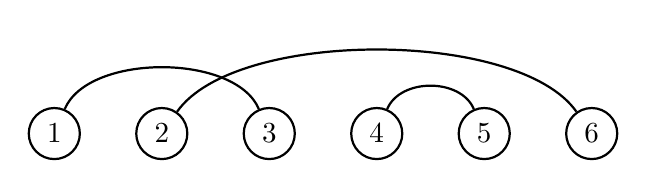
\begin{tikzpicture}[node distance={13mm}, thick, main/.style = {draw, circle, scale=1.05}]  
            \node[main] (1) {$1$};
            \node[main] (2) [right of=1] {$2$};
            \node[main] (3) [right of=2] {$3$};
            \node[main] (4) [right of=3] {$4$};
            \node[main] (5) [right of=4] {$5$};
            \node[main] (6) [right of=5] {$6$};
            
            
            \draw (1) to [out=67,in=113,looseness=0.8] (3);
            \draw (2) to [out=55,in=125,looseness=0.65] (6);
            \draw (4) to [out=67,in=113,looseness=1] (5);
        \end{tikzpicture}
    \end{center}
    \caption{The matching $m = \{(1,3),\; (2,6),\; (4,5)\}$.}
    \label{fig:matching example introduction}
\end{figure}

Note that $N \notin \Short(m)$ for every $m \in \M_N$. This holds even where $(1,N) \in m$.



Enumerative properties of short chords in perfect matchings were studied extensively. The distribution of the number of short chords in perfect matchings appears in entry A079267 of the OEIS~\cite{oeis}, and was analyzed for example by Cameron and Killpatrick~\cite{killpatrick2020statistics}. McSorley and Feinsilver~\cite{bessel_polynomials_mathcings} discovered that short chords of matchings are closely related to Bessel polynomials, as will be discussed in Section~\ref{subsec:schur coefficients bessel}.

The study of short chords of matchings is also motivated by the involutive length and its corresponding poset studied by Adin, Postnikov and Roichman~\cite{gelfand_involutions}. Related posets derived from the Bruhat order were studied by Richardson and Springer~\cite{richardson1990bruhat}, Hultman~\cite{hultman2008twisted}, Deodhar and Srinivasan~\cite{deodhar2001statistic} and others, motivated by the topology of linear algebraic groups (see~\cite{hultman2008twisted} for details). Further discussion on the algebraic motivations can be found in Section~\ref{subsec:schreier graph of perfect matchings}.




We prove the following:
\begin{theorem}
\label{thm:matchings schur positive}
    Let $n,f \in \NN$ be nonnegative integers, and denote $N=2n+f$. Then the set $\M_{N,f}$ is Schur-positive with respect to $\Short$. Furthermore, its Schur expansion is given by the following formula:
    \[
        \Q_{\Short} (\M_{N,f}) = \sum_{k=0}^n |\{ m\in \M_{N-2k,f} \mid \Short(m) = \emptyset\}|\ s_{N-k,k}.
    \]
\end{theorem}

It turns out  that the Schur coefficients of $\Q_{\Short} (\M_{N,f})$ 
may be explicitly interpreted in terms of Bessel polynomials, see 
Corollary~\ref{cor:schur expansion bessel} 
below.




We give two proofs of Theorem~\ref{thm:matchings schur positive}. The first proof relies on a new criterion for Schur-positivity of sparse statistics:

\begin{definition}
\label{def:sparse}
    We say that a set $J \subseteq [N-1]$ is \emph{sparse} if $\{j,j+1\} \nsubseteq J$ for every $1 \le j \le N-2$.

    For a set $\A$ and a function $D:\A \to 2^{[N-1]}$, we say that $D$ is \emph{sparse} if $D(a)$ is sparse for all $a \in \A$.
\end{definition}

\begin{theorem}
\label{thm:criterion schur positive two rows}
    Let $\A$ be a finite set with a statistic $D:\A \to 2^{[N-1]}$, and denote $n = \lfloor\frac{N}{2} \rfloor$. Then the following statements are equivalent:
    \begin{itemize}
        \item $D$ is sparse, and for every sparse $J \subseteq [N-1]$, the cardinality of the set $\{a \in \A \mid D(a) \supseteq J\}$ depends on the size of $J$ only.
        \item $\A$ is symmetric with respect to $D$, with a Schur expansion of the form $\Q_{D}(\A) = \sum_{k=0}^n c_k s_{N-k,k}$ for some $c_k \in \ZZ$.
    \end{itemize}

    Furthermore, if these statements hold then $\A$ is Schur-positive, and its Schur expansion is
    \[
        \Q_{D} (\A) = \sum_{k=0}^n \left|\left\{ a\in \A \mid D(a) = \{1,3,5,\dots, 2k-1\} \right\}\right|\: s_{N-k,k}.
    \]
    
\end{theorem}

This new criterion implies Theorem~\ref{thm:matchings schur positive}, %
as shown at the beginning of Section~\ref{sec:short chords in matchings}, and can be applied to many other sets as well.
It is also applied in a subsequent paper \cite{gallai} to prove Schur-positivity of Gallai colorings and transitive colorings of complete graphs.

The second proof of Theorem~\ref{thm:matchings schur positive} provides a bijection from the set of matchings to a multiset of SYTs,
and applies the bijective criterion of Adin and Roichman for Schur-positivity \cite[Prop.\ 9.1]{adin_roichman_fine_set}, presented in Theorem~\ref{thm:criterion schur positive young}.

Following the bijective proof, we present an equivalence relation on matchings, motivated by Knuth equivalence of permutations~\cite{knuth1970permutations}:
\begin{definition}\label{def:knuth like equivalence}
    We say that two matchings $m_1,m_2 \in \M_N$ are \emph{Knuth equivalent} if one can be obtained from the other by a sequence of \emph{elementary Knuth transformations}:
    \begin{itemize}
        \item Replace the chords $(i,i+1),\; (i+2)$ with the chords $(i),\; (i+1,i+2)$ or vice versa (\ie interchange a short chord with an adjacent unmatched vertex).
        \item Replace the chords $(i,i+1),\; (i+2,j)$ with the chords $(i,j),\; (i+1,i+2)$, or $(i,i+1),\; (j,i+2)$ with $(j,i),\; (i+1,i+2)$, or vice versa (\ie interchange a short chord with an adjacent endpoint of another chord).
    \end{itemize}
\end{definition}

We also define the core of a given matching:

\begin{definition}[Definition~\ref{def:core of matching} below]
    The \emph{core} of a given matching $m \in \M_N$, denoted $\core(m)$, is obtained by repeatedly removing short chords from the matching until no short chords remain. The remaining vertices are then re-indexed with natural numbers starting from $1$ while preserving their relative order.

\end{definition}

A classical result due to Knuth~\cite{knuth1970permutations} states that two permutations $\pi_1,\pi_2 \in S_N$ are Knuth equivalent if and only if $P(\pi_1) = P(\pi_2)$, where $P(\pi)$ denotes the insertion tableau of a permutation $\pi$ defined by the Robinson-Schensted correspondence (see \cite[Section 3]{sagan_book} for details). We prove the following analogous result for matchings:
\begin{theorem}[Theorem~\ref{thm:knuth like equivalent iff same core} below]
    Two matchings $m_1, m_2 \in \M_N$ are Knuth equivalent if and only if $\core(m_1) = \core(m_2)$.
\end{theorem}

We show that Knuth classes of matchings, similarly to Knuth classes of permutations, have Schur functions as their generating functions:

\begin{theorem}[Corollary~\ref{cor:closed under knuth like is schur positive} below]
    Every set $\M \subseteq \M_N$ of matchings that is closed under Knuth equivalence is Schur-positive with respect to $\Short$. Moreover, if $\M$ is a Knuth equivalence class, then its generating function is $\Q_{\Short}(\M) = s_{N-k,k}$, where $N-2k$ is the number of vertices of $\core(m)$ for some arbitrary matching $m \in \M$.
\end{theorem}

Furthermore, utilizing Knuth classes, we explore in Section~\ref{sec:refinements} various refined Schur-positive sets, including:
\begin{itemize}
    \item The set of $k$-crossing matchings (\ie where $k$ is the maximal cardinality of a set of pairwise intersecting chords).
    \item The set of matchings with exactly $k$ pairs of intersecting chords.
\end{itemize}

Lastly, we define $\M_{N,f}(m)$ as the set of matchings in $\M_{N,f}$ that avoid the pattern $m$. In Proposition~\ref{prop:characterize pattern avoiding schur positive singletons}, we provide a characterization of the matchings $m$ for which $\M_{N,f}(m)$ is Schur-positive for all $N$ and $f$.

The remainder of this work is organized as follows: Section~\ref{sec:preliminaries} provides necessary background. In Section~\ref{sec:criterion two rows}, we prove a necessary and sufficient criterion for sparse Schur-positivity (Theorem~\ref{thm:criterion schur positive two rows}). In Section~\ref{sec:short chords in matchings}, we focus on matchings. We first derive the Schur-positivity of short chords in matchings (Theorem~\ref{thm:matchings schur positive}) from the above criterion. Then, we present an alternative bijective proof, followed by a description of the Schur coefficients of matchings in terms of Bessel polynomials. In Section~\ref{sec:refinements}, we utilize the bijection to refine the Schur-positivity property of Theorem~\ref{thm:matchings schur positive}. Finally, Section~\ref{sec:further research} concludes with further remarks and open problems.

\section{Preliminaries and notation}
\label{sec:preliminaries}

\begin{definition}
    For nonnegative integers $i,j$, we define the \emph{interval}
    \[
        [i,j] :=
        \begin{cases}
            \{i,i+1,\dots,j\} & \text{if $i \le j$,}\\
            \emptyset & \text{otherwise.}
        \end{cases}
    \]
    We also define $[i] = [1,i]$.
\end{definition}

\begin{definition}
\label{def:elements with given stat}
    Given a set $\A$, a function $D:\A \to 2^{[N-1]}$ and a set $J \subseteq [N-1]$, we denote $\A(D=J) := \{a \in \A \mid D(a) = J\}$ and $\A(D \supseteq J) := \{a \in \A \mid D(a) \supseteq J\}$.
\end{definition}

\subsection{Symmetric and quasisymmetric functions}
\label{subsec:definitions symmetric functions}

\begin{definition}
    Given $N \in \NN$, a \emph{partition} $\lambda$ of $N$ (denoted $\lambda \vdash N$), is a weakly-decreasing sequence $\lambda = (\lambda_1 \ge \lambda_2 \ge \dots \ge \lambda_\ell)$ of positive integers, such that $\lambda_1 + \dots + \lambda_\ell = N$. The values $(\lambda_1,\dots,\lambda_\ell)$ are called the \emph{parts} of $\lambda$.
    
    A \emph{composition} $\alpha$ of $N$ (denoted $\alpha \vDash N$) is a sequence $\alpha = (\alpha_1, \alpha_2, \dots, \alpha_\ell )$ of positive integers, such that $\alpha_1 + \dots + \alpha_\ell = N$. Every partition is a composition.
\end{definition}

Compositions of $N$ are in bijection with subsets of $[N-1] := \{1, \dots, N-1\}$ by 
\[
    [N-1] \supseteq \{i_1, i_2, \dots, i_\ell \} \mapsto (i_1, i_2 - i_1, \dots, i_\ell - i_{\ell-1}, N - i_\ell) \vDash N.
\]
For example, for $N = 10$, $\{2, 4, 7, 8\} \mapsto (2, 2, 3, 1, 2)$. The composition associated to a set $S$ is denoted $\alpha_S$, and the set associated to a composition $\alpha$ is denoted $S_\alpha$.

We say that two compositions $\alpha, \beta \vDash N$ are \emph{equivalent} (denoted $\alpha \sim \beta$), if $\beta$ is a rearrangement of the entries of $\alpha$.

Denote the ring of symmetric functions by $\sym$ and the ring of quasisymmetric functions by $\qsym$ (see, for example, \cite[Section 1]{S3_patterns_list} for details). The space of homogeneous symmetric functions of degree $N$ is denoted by $\sym_N$, and the space of homogeneous quasisymmetric functions of degree $N$ is denoted by $\qsym_N$.

The space $\qsym_N$ has several important bases. In this work, we focus on the \emph{fundamental basis}, consisting of the functions
\[
    F_{N,S} := \sum_{\substack{i_1 \le i_2 \le \dots \le i_N \\ \forall j \in S:i_j < i_{j+1}}} x_{i_1} x_{i_2} \dots x_{i_N},\quad S \subseteq [N - 1].
\]
We write $F_S$ instead of $F_{N,S}$ when $N$ is clear from the context.

The space $\sym_N$ has several standard bases as well. In this work, we focus on the Schur basis, which consists of the Schur functions $s_{\lambda}$, where $\lambda$ is a partition of $N$. 
The definition and properties of Schur functions can be found in \cite[Section 4.4]{sagan_book}. Here, we adopt the combinatorial approach to Schur functions, as described in Theorem~\ref{thm:schur functions young tableaux} and Theorem~\ref{thm:criterion schur positive young} below.

\subsection{Symmetric and Schur-positive sets}
\label{subsec:schur positive sets}
As mentioned in Section~\ref{sec:introduction}, a set $\A$ is symmetric with respect to a statistic $D:\A \to 2^{[N-1]}$ if the generating function $\Q_{D}(\A)$ is a symmetric function. Moreover, it is Schur-positive if all Schur coefficients are nonnegative integers.


One of the fundamental constructions of Schur-positive sets, regarding sets of standard Young tableaux (SYT), is due to Gessel~\cite{knuth_classes_schur_positive}. Let $\Syt(\lambda)$ denote the set of standard Young tableaux of shape $\lambda$. We draw tableaux in English notation, as in Figure~\ref{fig:SYT example}. The \emph{descent set} of $T\in \Syt(\lambda)$ is
\[
    \Des(T) := \{i \in [N-1] \mid i+1 \text{ appears in a lower row than $i$ in $T$}\}.
\]
For example, the descent set of the SYT in Figure~\ref{fig:SYT example} is $\{2,4,7,8\}$.

